\documentclass[xelatex]{beamer}

% 算法,伪代码
\usepackage{latexsym}
\usepackage{amsmath,amssymb,bm}
\usepackage{color,xcolor,tikz}
\usepackage{algorithm,algorithmic}
\usepackage{amsthm}
\floatname{algorithm}{算法}
\renewcommand{\algorithmicrequire}{\textbf{输入:}} 
\renewcommand{\algorithmicensure}{\textbf{输出:}}

\mode<presentation> {

\usetheme{Madrid}
\usefonttheme[onlymath]{serif}
\setbeamertemplate{footline}[page number] 
\setbeamertemplate{navigation symbols}{} 
}

\usepackage[UTF8]{ctex}     
\graphicspath{{graphics/}}     
\DeclareGraphicsExtensions{.eps,.png,.jpg} 
\CTEXoptions[today=old]


\AtBeginSection[] { 
  \begin{frame}
    \frametitle{Outline} 
    \tableofcontents[currentsection] 
  \end{frame} 
  \addtocounter{framenumber}{-1}  %目录页不计算页码
}
%--------------------------------------------------------------
%	TITLE PAGE
%--------------------------------------------------------------
\title[]{Wasserstein Generative Adversarial Nets} 
% \subtitle{}
\author{Presented by Yang Xue} 
\institute[SCU] 
{
Sichuan University \\ 
\medskip
% \textit{john@smith.com} % Your email address
}
\date{\today} 
%---------------------------------------------------------------




\begin{document}

%----------------------------------------------------------------
\begin{frame}
\titlepage 
\end{frame}
%\begin{frame}
%\frametitle{Overview} 
%\tableofcontents 
%\end{frame}
%----------------------------------------------------------------


%----------------------------------------------------------------
%	PRESENTATION SLIDES
%----------------------------------------------------------------

%------------------------------------------------
\section{GAN 存在的问题}
%------------------------------------------------
%\subsection{KL-散度的优化}

\begin{frame}
  \frametitle{KL-散度的优化}
  \begin{columns}[t]
    \column{.45\textwidth}
    \textbf{KL-散度:}
    $$
    KL \left (\mathbb{P}_r \parallel \mathbb{P}_{g_\theta} \right ) = \int_{\chi}p_r(x) log \frac{p_r(x)}{p_g(x)}
    $$
    \textbf{不对称性:}
    $$
    KL \left (\mathbb{P}_r \parallel \mathbb{P}_g \right ) \neq KL \left (\mathbb{P}_g \parallel \mathbb{P}_r \right )
    $$
    \textbf{影响:$\nabla_\theta KL \left (\mathbb{P}_r \parallel \mathbb{P}_{g_\theta} \right ) = $}
      \begin{equation*}\begin{split}
        & = \int_{\chi} \nabla_\theta \left [ p_r(x) log(p_r(x)) - p_r(x) log(p_{g_\theta}(x)) \right ]dx \\
                 & = -\int_{\chi} \nabla_\theta \left [p_r(x) log(p_{g_\theta}(x)) \right ]dx   = -\int_{\chi} \left [\frac{p_r(x)}{p_g(x)} \nabla_\theta p_{g_\theta}(x) \right]dx  \\
                 & = -\int_{\chi_A} \left [\frac{p_r(x)}{p_g(x)} \nabla_\theta p_{g_\theta}(x) \right]dx - \int_{\chi_B} \left [\frac{p_r(x)}{p_g(x)} \nabla_\theta p_{g_\theta}(x) \right]dx
      \end{split}
      \end{equation*}

    \column{0.5\textwidth}
    \textbf{例子:}
      \begin{figure}
      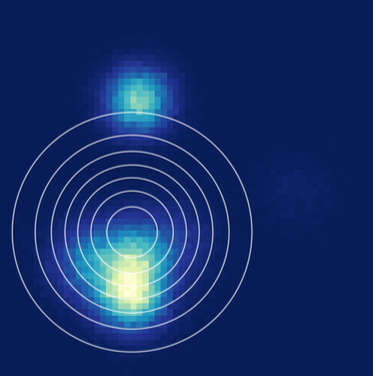
\includegraphics[width=0.65\linewidth]{kld}
      \end{figure}
  \end{columns}
\end{frame}
%------------------------------------------------
\subsection{生成器梯度消失}
\begin{frame}
\frametitle{完美判别器}
\begin{columns}[t]
  \column{.45\textwidth}
    %\textbf{KL-散度有意义的前提条件:}
    %\begin{enumerate}
    %  \item $\mathbb{P}_r$和$\mathbb{P}_{g_\theta}$在数据空间$\chi$上重叠。
    %\end{enumerate}
    %\vspace{2mm}
    \textbf{真实的数据分布情况:} \\
    \begin{enumerate}
      \item $\mathbb{P}_r$分布在$\chi$的低维流形上。
      \item $\mathbb{P}_g$也在$\chi$的低维流形上。
    \end{enumerate}
    \vspace{3mm}
    \textbf{结论:} \\
    \begin{enumerate}
      \item $\mathbb{P}_r$和$\mathbb{P}_{g_\theta}$在$\chi$是离散的。
      \item $\mathbb{P}_r$和$\mathbb{P}_{g_\theta}$在$\chi$几乎不重叠的。
      % \item KL-散度,JS-散度在没法提供有意义的梯度。
    \end{enumerate}
    \begin{theorem}[完美判别器]
      存在一个光滑的判别器 $D^*$ 使得$\mathbb{P}_r[D^*(x) = 1] = 1,\mathbb{P}_g[D^*(x) = 0] = 1$,且$\nabla_xD^*(x) = 0$。
    \end{theorem}

    \column{.45\textwidth}
    \textbf{实验的情况:} \\
      \begin{enumerate}
        \item 训练一开始loss迅速降为0。
        \vspace{2mm}
        \item 判别器趋于“完美判别器”,由$loss = \mathbb{E}_{x \sim \mathbb{P}_r}[logD(x)] + \mathbb{E}_{x \sim \mathbb{P}_g}[log(1-D(x))]$)
        \vspace{2mm}
        \item \uline{一旦出现完美判别器情况,就无法训练。}
      \end{enumerate}
  \end{columns}
  
\end{frame}
%------------------------------------------------
\begin{frame}
\frametitle{生成器梯度消失}
\begin{theorem}
  在之前的假设下:
  $$
  \lim_{\left \| D - D^* \right \| \to 0} {\nabla}_{\theta} \mathbb{E}_{z \sim p(z)} \left [ log(1 - D(g_{\theta}(z))) \right ] = 0
  $$
\end{theorem}
\vspace{5mm}
${\left \| {\nabla}_{\theta} \mathbb{E}_{z \sim p(z)} \left [ log(1 - D(g_{\theta}(z))) \right ] \right \|}_2^2$ 
\begin{equation*}\begin{split}
& <   \mathbb{E}_{z \sim p(z)} \left [  \frac{\left ( {\left \| \nabla_{\theta}D^*(g_{\theta}(z)) \right \| }_2 + \epsilon  \right )^2 {\left \| J_{\theta}g_{\theta}(z) \right \|}_2^2}{\left ( \left | 1 - D^*(g_{\theta}(z)) \right | - \epsilon  \right  )^2} \right ]    \\
& = \mathbb{E}_{z \sim p(z)} \left [ \frac{{\epsilon }^2 \left \| J_{\theta (z)} \right \|^2_2}{\left ( 1 - \epsilon  \right )^2}  \right ]   \\
& \leq M^2 \frac{\epsilon ^ 2}{(1 - \epsilon)^2}
\end{split}\end{equation*}

\end{frame}

\begin{frame}
  \frametitle{梯度消失-举例}
  \begin{example}[分布的支撑集不重叠导致梯度消失]
    对于数据空间中的任意一点 $x$ 只可能有下面4种情况:
    \begin{enumerate}
      \item $p_{r}(x) = 0$ 且 $p_{g}(x) = 0$ \label{a}
      \item $p_{r}(x) \neq 0$ 且 $p_{g}(x) \neq 0$ \label{b}
      \item $p_{r}(x) \neq 0$ 且 $p_{g}(x) = 0$ \label{c}
      \item $p_{r}(x) = 0$ 且 $p_{g}(x) \neq 0$ \label{d}
    \end{enumerate}
  \end{example}
  上面4项对 JS-散度计算的贡献:
  \begin{enumerate}
    \item \ref{a}项对JS-散度计算的贡献为0
    \item \ref{c}和\ref{d}项表示的是分布$\mathbb{P}_r$和$\mathbb{P}_g$不重叠的部分对JS-散度计算的贡献为常数$log2$
    \item \ref{b}项表示的是分布$\mathbb{P}_r$和$\mathbb{P}_g$重叠的部分,只有这一部分才能对生成器提供梯度
  \end{enumerate}
\end{frame}

%------------------------------------------------
\subsection{原始目标函数的训练不稳定}
\begin{frame}
  上例说明:如果分布$\mathbb{P}_r$和$\mathbb{P}_g$重叠的部分可以忽略不计则会出现梯度消失。
  而训练不稳定的根因正是梯度时而会消失。\\
  \vspace{2mm}
  根本原因:
  \begin{enumerate}
    \item 实际情况糟糕:分布基本不重叠,容易使判别器达到“完美”
    \item JS-散度,KL-散度在上面情况下不可靠(可能无法提供有效的梯度)
  \end{enumerate}
  \vspace{2mm}
  带来的问题:
  \begin{enumerate}
    \item 生成器和判别器的训练需要平衡
    \item 网络结构对结果影响很大(实验现象)
  \end{enumerate}
  解决办法:
  \begin{enumerate}
    \item 添加噪声,使添加噪声后的分布重叠,再逐渐退火
    \item 更换另一种距离,它能处理分布不重叠的情况
  \end{enumerate}
\end{frame}

%------------------------------------------------
\subsection{替换目标函数的训练不稳定}
\begin{frame}
\frametitle{替换目标函数的模型坍塌以及训练不稳定}
\begin{columns}[t]
  \column{.5\textwidth}
\textbf{替代目标函数:} \\
$$
\mathbb{E}_{z \sim p(z)} \left [-log(D(g_\theta(z))) \right]
$$
\column{.5\textwidth}
  \textbf{特点:}
  \begin{enumerate}
    \item 相同的不动点。
    \item 不再等价于优化 JS 散度。
  \end{enumerate}
\end{columns}
\begin{theorem}
  令$\mathbb{P}_r,\mathbb{P}_{g_\theta}$是两个连续的概率分布,它们的概率密度分别为$p_r,p_{g_\theta}$。固定$\theta = \theta_0$,令$D^* = \frac{p_r}{p_r + p_{g_{\theta_0}}}$为最优的判别器,则:
  $$
  \mathbb{E}_{z \sim p(z)} \left [ -\nabla_\theta log D^*(g_\theta(z)) \mid_{\theta=\theta_0} \right ] = \nabla_\theta \left [ KL \left (\mathbb{P}_{g_\theta} \parallel \mathbb{P}_r \right) - 2JSD\left (\mathbb{P}_{g_\theta} \parallel \mathbb{P}_r  \right )\right ] \mid_{\theta=\theta_0}
  $$
\end{theorem}
\vspace{4mm}
\textbf{可以看出:} \\
\begin{enumerate}
  \item 梯度更新不稳定(梯度服从柯西分布,期望和方差无限大)。
  \item 造成模型坍塌的问题。
  \item 倾向于生成高质量的图像。
\end{enumerate}
\end{frame}

%------------------------------------------------
\section{WGAN}
%------------------------------------------------

\subsection{最优传输距离}
\begin{frame}
\frametitle{什么是 EMD 距离}
\textbf{最优传输距离:}
\begin{figure}
  \includegraphics[width=0.65\linewidth]{EMD}
\end{figure}
$$
\mathit{W}(\mathbb{P}_r , \mathbb{P}_\theta) = \inf_{\gamma \in \Pi(\mathbb{P}_r, \mathbb{P}_\theta) }\mathbb{E}_{(x,y) \in \gamma }  \left [ \left \| x - y \right \| \right ]
$$
\begin{columns}[t]
  \column{.5\textwidth}
  \textbf{优点:}
    \begin{enumerate}
      \item 适用于测量支撑集不重叠的分布的距离。
      \item $\mathit{W}(\mathbb{P}_r , \mathbb{P}_\theta)$对$\theta$连续。
      %\item 倾向于生成高质量的图像。
    \end{enumerate}
  \column{.45\textwidth}
  \textbf{缺点:}
    \begin{enumerate}
      \item 计算复杂度高。
      %\item 
    \end{enumerate}
\end{columns}
\end{frame}
%------------------------------------------------

\begin{frame}
\frametitle{一个例子}
\begin{columns}[t]
  \column{.65\textwidth}
  \begin{example}[支撑集不重叠的分布之间的散度]
  令$\mathit{Z} \sim \mathit{U}[0,1]$,$\mathbb{P}_0 \sim (0, \mathit{Z})$,$\mathbb{P}_\theta \sim (\theta, Z)$,则:
  \begin{enumerate}
    \item $\mathit{W}(\mathbb{P}_r , \mathbb{P}_\theta) = |\theta|$
    \item 
    $
    JS(\mathbb{P}_r , \mathbb{P}_\theta) = 
    \begin{cases}
      log2 & \text{$\theta \neq 0$} \\
      0 & \text{$\theta = 0$}
    \end{cases}
    $
    \item $
    KL(\mathbb{P}_r , \mathbb{P}_\theta) = 
    \begin{cases}
      +\infty & \text{$\theta \neq 0$} \\
      0 & \text{$\theta = 0$}
    \end{cases}
    $
  \end{enumerate}
  \end{example}
  \column{.35\textwidth}
  \begin{figure}
    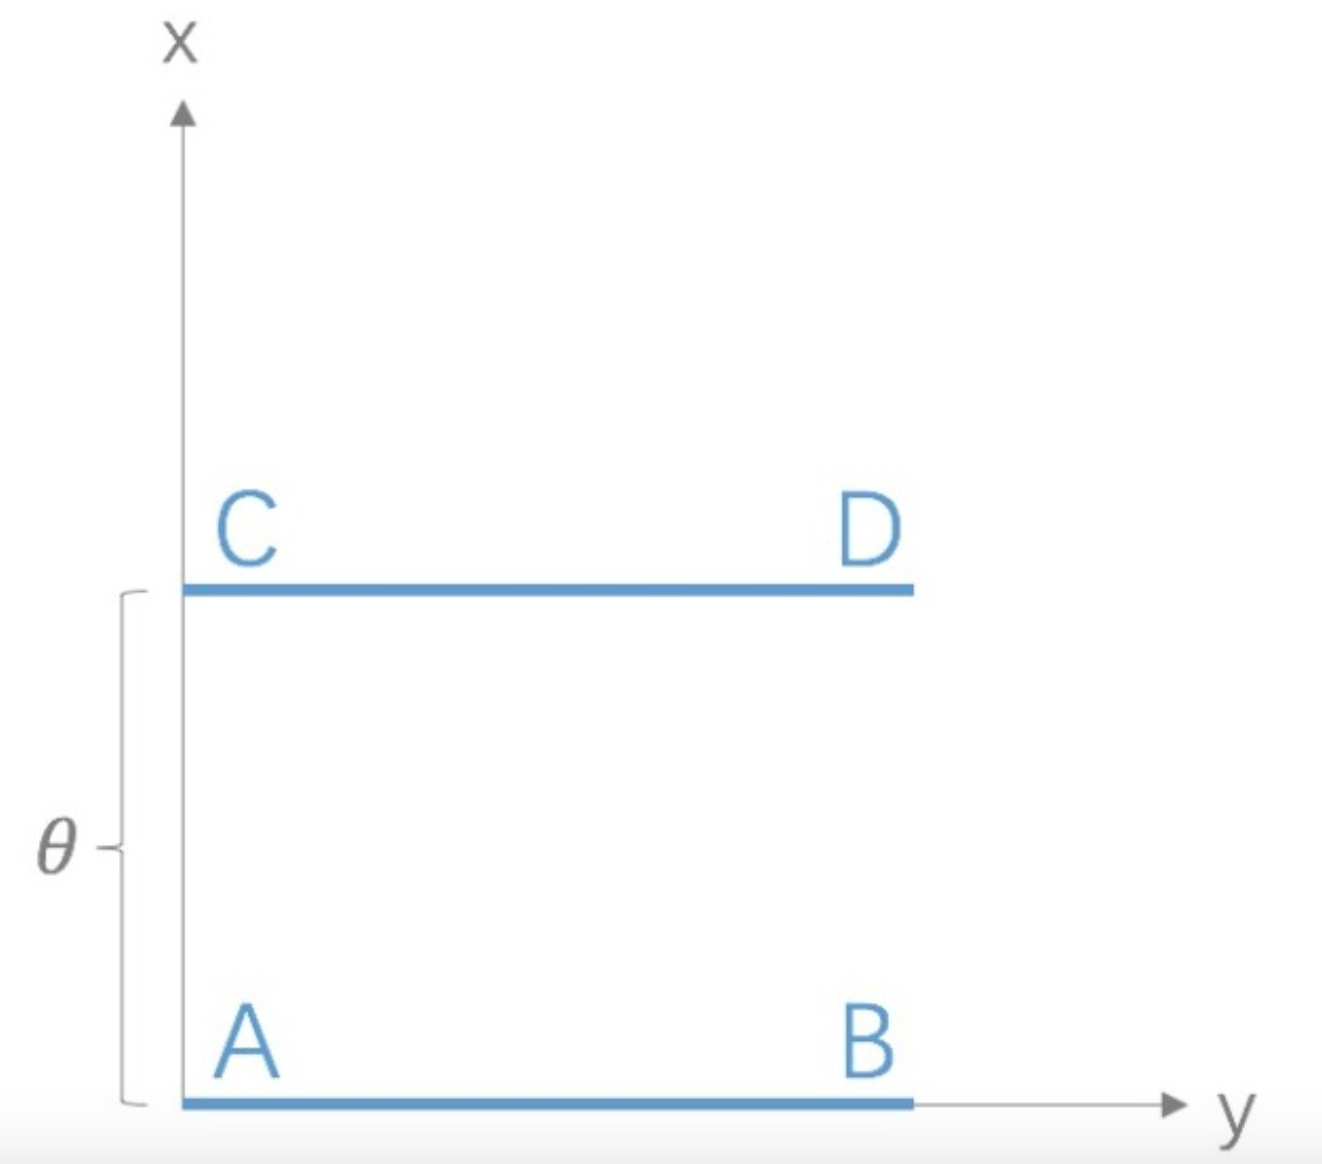
\includegraphics[width=0.65\linewidth]{example1}
  \end{figure}
\end{columns}
\textbf{上面的例子可以看出:}
\begin{enumerate}
  \item  KL 与 JS 散度不连续,无意义的梯度
  \item W 距离能提供梯度
\end{enumerate}
\begin{theorem}
  在一定的条件下,$\mathit{W}(\mathbb{P}_r , \mathbb{P}_\theta)$对$\theta$是连续的,且几乎处处可微。
\end{theorem}
\end{frame}

%------------------------------------------------
\subsection{W-距离的优化}

\begin{frame}
\frametitle{W-距离的优化}
\textbf{W-距离的对偶形式:}
\begin{equation*}
  \begin{split}
    \mathit{W}(\mathbb{P}_r , \mathbb{P}_\theta) &= \sup_{\left \| f \right \|_{L} \leq 1} \mathbb{E}_{x \sim \mathbb{P}_r} \left [ f(x) \right ] - \mathbb{E}_{x \sim \mathbb{P}_\theta} \left [ f(x) \right ] \\
    &= \sup_{\left \| f \right \|_{L} \leq 1} \mathbb{E}_{x \sim \mathbb{P}_r} \left [ f(x) \right ] - \mathbb{E}_{z \sim \mathbb{P}_{g_\theta}} \left [ f(g_\theta(z)) \right ]
  \end{split}
\end{equation*}

\begin{algorithm}[H]                    
  \caption{WGAN}         
  \begin{algorithmic}  
    \STATE Sample $\left \{ x^{(i)}) \right \}^m_{i=1} \sim \mathbb{P}_r$
    \STATE Sample $\left \{ z^{(i)}) \right \}^m_{i=1} \sim \mathbb{P}_z$
    \STATE $\Delta \omega \leftarrow \nabla_{\omega} \left [ \frac{1}{m}\sum_{i=1}^{m} f_{\omega }(x^{(i)}) - \frac{1}{m}\sum_{i=1}^{m} f_{\omega }(g_\theta(z^{(i)})) \right ]$
    \STATE $\omega \leftarrow \omega + \eta \cdot \Delta \omega$
    \STATE $\omega \leftarrow clip(\omega, -c ,c)$
    \STATE Sample $\left \{ z^{(i)}) \right \}^m_{i=1} \sim \mathbb{P}_z$
    \STATE $\Delta \theta \leftarrow  - \nabla_{\theta} \left [\frac{1}{m}\sum_{i=1}^{m} f(g_\theta(z^{(i)})) \right ]$
    \STATE $\theta \leftarrow \theta - \eta \cdot \Delta \theta$
  \end{algorithmic}
\end{algorithm}
\end{frame}

\subsection{与原始 GAN 的区别}
\begin{frame}
  \frametitle{与原始 GAN 的区别}
  \begin{columns}[t]
  \column{.45\textwidth}
    \textbf{算法区别:}
    \begin{enumerate}
      \item 去掉了 D 最后一层的非线性 Sigmoid 函数。
      \item 去掉了目标函数里的 Log。
      \item D的权重被截断在$[-c, c]$之间。
    \end{enumerate}
  \column{.45\textwidth}
    \textbf{提升:}
    \begin{enumerate}
      \item 训练稳定,不需要平衡 G 和 D 的能力。
      \item 没有模型坍塌,图片效果更好。
      \item 有意义的 loss 测量。
    \end{enumerate}
  \end{columns}
  \vspace{4mm}
  \textbf{有意义的 loss:}
  \begin{figure}
  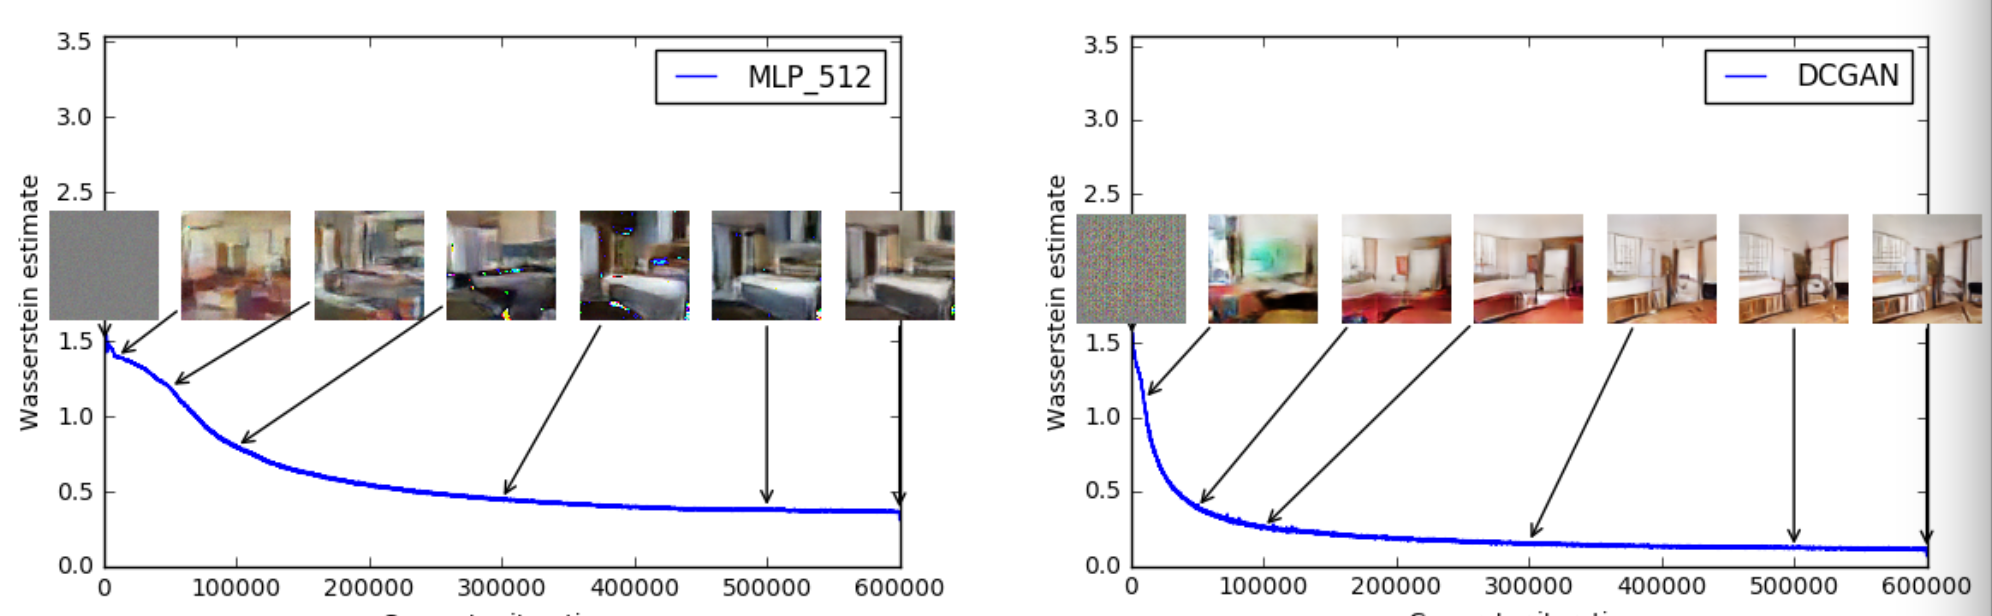
\includegraphics[width=0.65\linewidth]{w_estimate}
  \end{figure}
\end{frame}

%------------------------------------------------
\begin{frame}
\Huge{\centerline{The End}}
\end{frame}
%------------------------------------------------

\end{document} 